\chapter{Quelques fonctions importantes}

\section{Exponentielle et logarithme}

L'exponentielle est la seule fonction égale à sa dérivée. Elle correspond à l'exponentiation de la constante de Néper $e \approx 2.72$:

\begin{align}
    \exp(x) = e^x
\end{align}

La fonction exponentielle est une application continue et indéfiniment dérivable sur $\mathbb{R}$.\\


Le logarithme népérien est la primitive de la fontion $x \mapsto \frac{1}{x}$ sur l'intervalle $] 0,+\infty[$, qui s'annule en 1. Autrement dit,

\begin{align}
\ln :] 0, & +\infty[\rightarrow \mathbb{R} \\
x & \mapsto \int_1^{\mathbf{x}} \frac{\mathbf{d t}}{\mathbf{t}}
\end{align}

La fonction ln est une application continue, strictement croissante et indéfiniment dérivable sur l'intervalle $] 0,+\infty[$

\thmr{Propriétés de l'exponentielle}{exp}{
    \begin{align}
        \forall x \in \mathbb{R}, \exp ^{\prime}(x)&=\exp (\mathbf{x})\\
        \forall(x, y) \in \mathbb{R}^2, e^{x+y}&=\mathbf{e}^{\mathbf{x}} \mathbf{e}^{\mathbf{y}}\\
        \forall(x, y) \in \mathbb{R}, e^{x-y}=\frac{\mathbf{e}^{\mathbf{x}}}{\mathbf{e}^{\mathbf{y}}}\\
        \forall(x, a) \in \mathbb{R} \times \mathbb{Z}, e^{a x}&=\left(\mathbf{e}^{\mathbf{x}}\right)^{\mathbf{a}}\\
        \forall x \in \mathbb{R}^{+*}, \exp (\ln (x))&=\mathbf{x}\\
        \forall x \in \mathbb{R}, \ln (\exp (x))&=\mathbf{x}
    \end{align}

}


\thmr{Propriétés du logarithme}{log}{
    \begin{align}
        \forall x>0, \ln ^{\prime}(x)&=\frac{1}{\mathrm{x}}\\
        \forall x>0, \forall y>0, \ln (x y)&=\ln (\mathbf{x})+\ln (\mathbf{y}) \\
\forall x>0, \forall n \in \mathbb{Z}, \ln \left(x^n\right)&=\mathbf{n} \ln (\mathbf{x})\\
\forall x>0, \ln \left(\frac{1}{x}\right)&=-\ln (\mathbf{x}) \\
\forall x>0, \forall y>0, \ln \left(\frac{x}{y}\right)&=\ln (\mathbf{x})-\ln (\mathbf{y})
    \end{align}
}

\subsection*{En base quelconque}
$$
\begin{aligned}
\exp _a: & \mathbb{R} \rightarrow] 0,+\infty[ \\
x & \mapsto a^x=\exp (x \ln (a))
\end{aligned}
$$

elle est définie comme la bijection réciproque du logarithme de base a.

Logarithme de base $\mathbf{n}$, défini $\forall n \in \mathbb{N}^*$ par

$$
\forall x>0, \log _n(x)=\frac{\ln (\mathbf{x})}{\ln (\mathbf{n})}
$$


En particulier, le logarithme de base $10, \log _{10}(x)=\frac{\ln (x)}{\ln (10)}$, est fréquemment utilisé (surtout pour les représentations graphiques).

ATTENTION: les notations courantes du logarithme de base 10 sont $\log _{10}, \log$, Log ou lg et celles du logarithme népérien, aussi appelé logarithme naturel sont $\ln$, ou log. Il y a donc ambiguité dans certaines situations. En programmation, généralement, la fonction log fait référence au logarithme népérien. 

\begin{figure}[H]
    \centering
    \begin{tikzpicture}
        \tzaxes(-3,-3)(3,3){$x$}{$y$}
        \tzfn[blue,thick]{exp(\x)}[-3:1]{$e^x$}[ar]
        \tzfn[black,thick]{(\x)}[-3:3]{$x$}[ar]
        \tzfn[red,thick]{ln(\x)}[0.1:3]{$\ln x$}[ar]
    \end{tikzpicture}
\end{figure}

\section{Fonctions puissance}

Ce sont les fonctions de la forme 

$$
f_a: x \mapsto x^a
$$

avec $a$ un nombre différent de 0.\\

\subsection*{Si $a$ est un entier}
Si $a$ est pair, $f_a$ est paire. Si $a$ est impair, $f_a$ est impaire.
L'allure générale de $f_a$ dépend de la parité de $a$ et de son signe.

\begin{figure}[H]
    \centering
    \begin{minipage}{0.45\textwidth}
        \begin{tikzpicture}
            \tzaxes(-3,-3)(3,3){$x$}{$y$}
            \tzfn[blue,thick]{(\x)^2}[-2:2]{$x^2$}[ar]
            \tzfn[red,thick]{(\x)^3}[-1.5:1.5]{$x^3$}[ar]
            \end{tikzpicture}
    \end{minipage}
    \hfill
    \begin{minipage}{0.45\textwidth}
        \begin{tikzpicture}
            \tzaxes(-3,-3)(3,3){$x$}{$y$}
            \tzfn[blue,thick]{(\x)^(-2)}[0.5:2.5]{$x^{-2}$}[ar]
            \tzfn[blue,thick]{(\x)^(-2)}[-0.5:-2.5][ar]
            \tzfn[red,thick]{(\x)^(-3)}[0.65:2.5]{$x^{-3}$}[ar]
            \tzfn[red,thick]{(\x)^(-3)}[-0.65:-2.5][ar]
            \end{tikzpicture}
    \end{minipage}
\end{figure}

\subsection*{Si $a$ est rationnel}

En particulier, si $a=\frac{1}{n}$ avec $n$ un entier naturel, alors $f_a$ est une fonction racine.

\begin{figure}[H]
    \centering
        \begin{tikzpicture}
            \tzaxes(0,0)(4,4){$x$}{$y$}
            \tzfn[blue,thick]{(\x)^(1/2)}[0:3]{$\sqrt[2]{x}$}[ar]
            \tzfn[red,thick]{(\x)^(1/3)}[0:4]{$\sqrt[3]{x}$}[ar]
            \tzfn[green,thick]{(\x)^(1/4)}[0:3]{$\sqrt[4]{x}$}[ar]
            \end{tikzpicture}
\end{figure}

\subsection*{Si $a$ est réel}

Toute fonction puissance peut être mise sous la forme
\begin{align}
    f_a: \mathbb{R}^{+*} \rightarrow \mathbb{R}^{+*} & \\
    & x \mapsto x^a=e^{a \ln (x)}
\end{align}

\section{Fonctions trigonométriques}
\thmr{Identités trigonométriques}{trigo}{

\begin{align}
    & \cos^2(\theta) + \sin^2(\theta) = 1 \\
& \cos \left(\theta_1+\theta_2\right)=\cos \theta_1 \cos \theta_2-\sin \theta_1 \sin \theta_2 \\
& \sin \left(\theta_1+\theta_2\right)=\sin \theta_1 \cos \theta_2+\cos \theta_1 \sin \theta_2 \\
& \cos \left(\theta_1-\theta_2\right)=\cos \theta_1 \cos \theta_2+\sin \theta_1 \sin \theta_2 \\
& \sin \left(\theta_1-\theta_2\right)=\sin \theta_1 \cos \theta_2-\cos \theta_1 \sin \theta_2\\
\tan \left(\theta_1+\theta_2\right) & =\frac{\tan \theta_1+\tan \theta_2}{\mathbf{1}-\tan \theta_1 \tan \theta_2} \\
\tan \left(\theta_1-\theta_2\right) & =\frac{\tan \theta_1-\tan \theta_2}{\mathbf{1}+\tan \theta_1 \tan \theta_2}\\
& \sin 2 x=\mathbf{2} \sin \mathbf{x} \cos \mathbf{x} \\
& \cos 2 x=\cos ^2 \mathbf{x}-\sin ^2 \mathbf{x}=\mathbf{2} \cos ^2 \mathbf{x}-\mathbf{1}=\mathbf{1}-\mathbf{2} \sin ^2 \mathbf{x} \\
& \tan 2 x=\frac{\mathbf{2} \tan \mathbf{x}}{\mathbf{1}-\tan ^2 \mathbf{x}}\\
\cos a \cos b & =\frac{\mathbf{1}}{\mathbf{2}}(\cos (\mathbf{a}+\mathbf{b})+\cos (\mathbf{a}-\mathbf{b})) \\
\sin a \sin b & =\frac{\mathbf{1}}{\mathbf{2}}(\cos (\mathbf{a}-\mathbf{b})-\cos (\mathbf{a}+\mathbf{b})) \\
\sin a \cos b & =\frac{\mathbf{1}}{\mathbf{2}}(\sin (\mathbf{a}+\mathbf{b})+\sin (\mathbf{a}-\mathbf{b}))\\
    & \cos p+\cos q=\mathbf{2} \cos \frac{\mathbf{p}+\mathbf{q}}{\mathbf{2}} \cos \frac{\mathbf{p}-\mathbf{q}}{\mathbf{2}} \\
    & \cos p-\cos q=-\mathbf{2} \sin \frac{\mathbf{p}+\mathbf{q}}{\mathbf{2}} \sin \frac{\mathbf{p}-\mathbf{q}}{\mathbf{2}} \\
    & \sin p+\sin q=\mathbf{2} \sin \frac{\mathbf{p}+\mathbf{q}}{\mathbf{2}} \cos \frac{\mathbf{p}-\mathbf{q}}{\mathbf{2}} \\
    & \sin p-\sin q=\mathbf{2} \cos \frac{\mathbf{p}+\mathbf{q}}{\mathbf{2}} \sin \frac{\mathbf{p}-\mathbf{q}}{\mathbf{2}}
\end{align}
}

\begin{figure}[H]
    \centering
    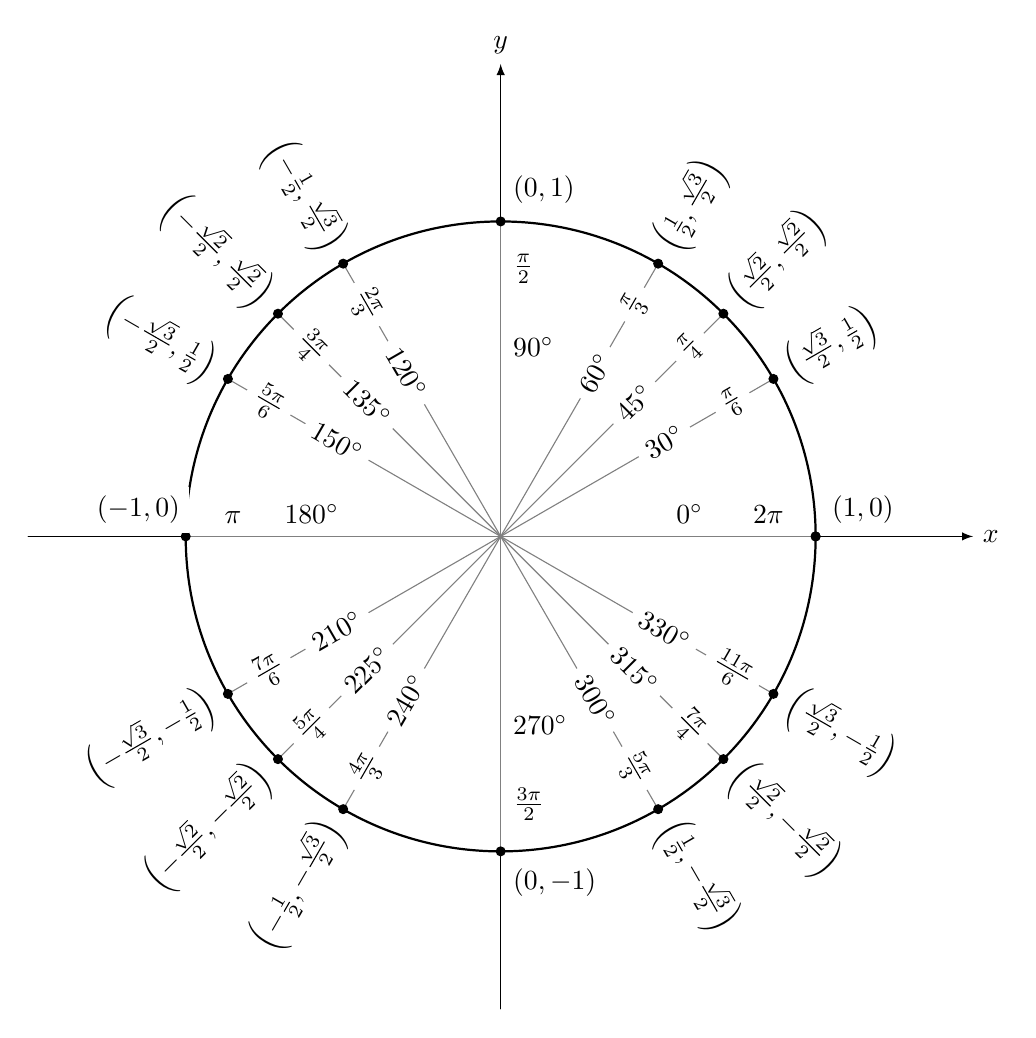
\begin{tikzpicture}[scale=4,cap=round,>=latex]
        \draw[->] (-1.5cm,0cm) -- (1.5cm,0cm) node[right,fill=white] {$x$}; % x axis
        \draw[->] (0cm,-1.5cm) -- (0cm,1.5cm) node[above,fill=white] {$y$}; % y axis
        
        % draw the unit circle
        \draw[thick] (0cm,0cm) circle(1cm);
        
        \foreach \x in {45,135, 225,315,0,30,...,360} { % <-- bissectrices added
          \draw[gray] (0cm,0cm) -- (\x:1cm); % lines from center to point
          \filldraw[black] (\x:1cm) circle(0.4pt); % dots at each point
        }
        
        % for the first and fourth quadrants
        \foreach \adeg/\radtext/\xc/\yc in {
          30/\frac{\pi}{6}/\frac{\sqrt{3}}{2}/\frac{1}{2},
          45/\frac{\pi}{4}/\frac{\sqrt{2}}{2}/\frac{\sqrt{2}}{2},
          60/\frac{\pi}{3}/\frac{1}{2}/\frac{\sqrt{3}}{2},
          300/\frac{5\pi}{3}/\frac{1}{2}/-\frac{\sqrt{3}}{2},
          315/\frac{7\pi}{4}/\frac{\sqrt{2}}{2}/-\frac{\sqrt{2}}{2},
          330/\frac{11\pi}{6}/\frac{\sqrt{3}}{2}/-\frac{1}{2}
        }
        {
          \draw (\adeg:0.6cm) node[fill=white, rotate around={\adeg:(0,0)}] {$\adeg^\circ$}; % <-- rotate around key used
          \draw (\adeg:0.85cm) node[fill=white, rotate around={\adeg:(0,0)}] {$\radtext$}; % <-- rotate around key used
          \draw (\adeg:1.025cm) node[fill=white, rotate around={\adeg:(0,0)}, anchor=west] {$\left(\xc,\yc\right)$}; % <-- rotate around key used, radius changed, anchor key used
        }
      
        % for the second and third quadrants
        \foreach \adeg/\radtext/\xc/\yc in {
          120 / \frac{2\pi}{3} / -\frac{1}{2} / \frac{\sqrt{3}}{2},
          135 / \frac{3\pi}{4} / -\frac{\sqrt{2}}{2} / \frac{\sqrt{2}}{2},
          150 / \frac{5\pi}{6} / -\frac{\sqrt{3}}{2} / \frac{1}{2},
          210 / \frac{7\pi}{6} / -\frac{\sqrt{3}}{2} / -\frac{1}{2},
          225 / \frac{5\pi}{4} / -\frac{\sqrt{2}}{2} / -\frac{\sqrt{2}}{2},
          240 / \frac{4\pi}{3} / -\frac{1}{2} / -\frac{\sqrt{3}}{2}
        }
        {
          \draw (\adeg:0.6cm) node[fill=white, rotate around={\adeg+180:(0,0)}] {$\adeg^\circ$}; % <-- rotate around key used
          \draw (\adeg:0.85cm) node[fill=white, rotate around={\adeg+180:(0,0)}] {$\radtext$}; % <-- rotate around key used
          \draw (\adeg:1.025cm) node[fill=white, rotate around={\adeg+180:(0,0)}, anchor=east] {$\left(\xc,\yc\right)$}; % <-- rotate around key used, radius changed, anchor key used
        }
        
        \foreach \adeg/\radtext/\xc/\yc in {0 / 2\pi / 1 / 0, 180 / \pi / -1 / 0}
        {
          \draw (\adeg:0.6cm) node[fill=white, above=1pt] {$\adeg^\circ$};
          \draw (\adeg:0.85cm) node[fill=white, above=1pt] {$\radtext$};
          \draw (\adeg:1.15cm) node[fill=white, above=1pt] {$\left(\xc,\yc\right)$}; % <-- radius changed
        }
        
        \foreach \adeg/\radtext/\xc/\yc in {90 / \frac{\pi}{2} / 0 / 1, 270 / \frac{3\pi}{2} / 0 / -1}
        {
          \draw (\adeg:0.6cm) node[fill=white, right=1pt] {$\adeg^\circ$};
          \draw (\adeg:0.85cm) node[fill=white, right=1pt] {$\radtext$};
          \draw (\adeg:1.1cm) node[fill=white, right=1pt] {$\left(\xc,\yc\right)$}; % <-- radius changed
        }
      \end{tikzpicture}
\end{figure}
\section{Fonctions hyperboliques}
Sinus hyperbolique
\begin{align}
\sinh : \mathbb{R} & \rightarrow \mathbb{R} \\
x & \mapsto \frac{\exp (x)-\exp (-x)}{2}
\end{align}

Cosinus hyperbolique
\begin{align}
\cosh : \mathbb{R} & \rightarrow[1,+\infty[ \\
x & \mapsto \frac{\exp (x)+\exp (-x)}{2}
\end{align}

Tangente hyperbolique
\begin{align}
\tanh & : \mathbb{R} \rightarrow]-1,1[ \\
& x \mapsto \frac{\sinh (x)}{\cosh (x)}=\frac{\exp (x)-\exp (-x)}{\exp (x)+\exp (-x)}
\end{align}

\begin{figure}[H]
    \centering
    \begin{tikzpicture}
        \tzaxes(-3,-3)(3,3){$x$}{$y$}
        \tzfn[blue,thick]{sinh(\x)}[-2:2]{$\sinh x$}[ar]
        \tzfn[red,thick]{cosh(\x)}[-1.5:1.5]{$\cosh x$}[ar]
        \tzfn[green,thick]{tanh(\x)}[-3:3]{$\tanh x$}[ar]
    \end{tikzpicture}
\end{figure}

\thmr{Identité hyperbolique}{hyp}{
    \begin{align}
        \forall x \in \mathbb{R}, \cosh ^{2}(x)&-\sinh ^{2}(x)=1
    \end{align}
}

\section{Croissances comparées}